\documentclass[]{article}
\usepackage{graphicx}
\usepackage{float}
\usepackage{caption}
\usepackage{subcaption}
\usepackage[export]{adjustbox}


% Title Page
\title{Fire Detection Neural Network Project}
\author{Viviane Becker}


\begin{document}
\maketitle
\newpage
\tableofcontents
\newpage

\section{Introduction}
For successful completion of the Data Scientist Bootcamp from KnowledgeHut a capstone project needs to be worked on showing the abilities to put the learned methods into practise.\\
In the guide handed over to us there were ten projects described which we could choose from or we could come up with our own project.\\
I decided to take the project which is described in the next section of this document as I am really fond of experimenting with Neural Networks.
	
\section{Problem Description Fire Detection}
Fire outbreaks in forests are a huge threat to human and animals and are as well destroying nature that might have taken years to develop. Hence some prevention system is necessary to stop these outbreaks as soon as possible.\\
Traditional systems like temperature or smoke sensors are costly and have a slow response time if the fire outbreak is not in reach of the sensors.\\
As an alternative to a traditional system the idea is to take images or videos from the forests that should be analyzed with Deep Learning methods to detect fire or smoke in the images.\\
In this project I was given a dataset of images, already devided in test and train data, which consist of three folders each representing the three classes "fire", "Smoke" and "non fire". The task is to build a neural network model which is able to correctly classify these images and tune it further to get better results.\\


\section{Development Environment}
Finding a suitable development environment was one of the biggest issues during this project.\\
I first tried to setup my own laptop which has a built-in NVIDIA GeForce RTX 2060 and hence should be suitable for training a neural network with TensorFlow on the GPU.\\
Unfortunately setting up TensorFlow is not as easy as it may sound. It took me hours to get TensorFlow to recognize my GPU and use it for training. A small MNIST problem did run through without any issues. So I started developing the code for the project in PyCharm. When I was finally able to read in all images and run my initial model the code was failing after some time having memory issues. I tried my best to solve it by decreasing the batch\_size and the image\_size, but the issue won't resolve. So I needed to switch to some other environments.\\
First I tried CoLab. I needed to upload the whole dataset to my GoogleDrive and mount the folder in CoLab to start training. Uploading the 6.5GB dataset took hours and when I was finally able to start training it was super slow due to the data connection. So I needed to download the data from GoogleDrive to my instance in CoLab. After finally handling this I realized that CoLab disconnects the instance as soon as you are inactive and if you reconnect to it again the data is lost and need to be uploaded again. I got the final blow from CoLab when it said to me on the second day of my trials with CoLab that I could not get a GPU anymore. Trying a training with CPU quickly showed that it would take too much time to train the network. So CoLab turned out to be useless to me.\\
Afterwards I tried out Gradient Paperspace environment. I could setup a private Dataset by uploading the data to its interface. But here was the problem. The free account just allowed you a maximum of 5GB storage space. Also the free GPUs were completely used up so I could only decide for a paid one. But only a real subscription would have solved my problem with the 5GB storage space. So again not useable for me. Otherwise it would have been a great tool to work with.\\
Finally a colleague of mine came to my rescue. He remembered that kaggle is allowing 30 hours free usage of GPU in a week. And it was easy to upload the dataset to it as a private dataset. The upload was much faster then before to GoogleDrive and I could upload a zip file which was automatically unzipped before creating the dataset. So whenever I started my notebook I was able to download the dataset in a rather short amount of time and use it directly. Still there were some limitations on kaggle. The memory, CPU and GPU were quite descent but were still limiting me in the batch\_size and image\_size I could run my training. So I did not play much with these two parameters happy that I was finally able to train my network. Also kaggle does only support programming in one single jupyter notebook (as far as I could discover). So my try to modularize my code and make it cleaner and structured needed to be reverted. All code was just put into one single notebook. But yes I was finally able to train the network and the training took a descent amount of time so I was able to try out new things to tune the network. Thank you kaggle for being my saviour!\\
PLEASE BE AWARE THAT ALL PATH ARE IN KAGGLE NOTATION! IT WILL NOT WORK IN ANOTHER ENVIRONMENT!


\section{Data Exploration}
The dataset consists out of a three classes: "fire", "non fire" and "Smoke".\\
First I had a look at the class frequencies to detect whether there have been any disbalances between the three classes. As you can see in the following picture it is super balanced, having exactly the same number of images per class in train and test dataset.\\
\begin{figure}[H]
	\centering
	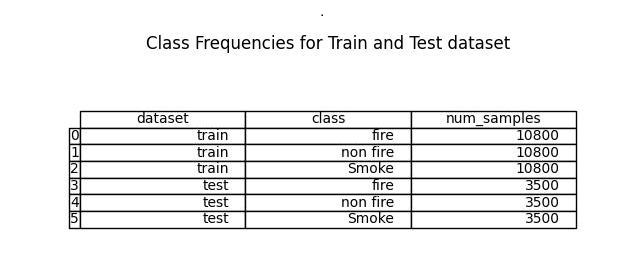
\includegraphics[width=0.9\textwidth]{"../visualizations/data_insights/class_frequencies_original.jpg"}
	\label{fig: class frequncies in test and train dataset}
\end{figure}
After making sure that the classes are not inbalanced I had a look at the height and width of the images. For this I calculated the width and height of each image and plottet it has a histogram showing how many images are having which height or width. You can see the results in the following images:\\
\begin{figure}[H]
	\centering
	\begin{subfigure}{0.45\textwidth}
		\caption{"Histogram showing how frequent which height in the images are"}
		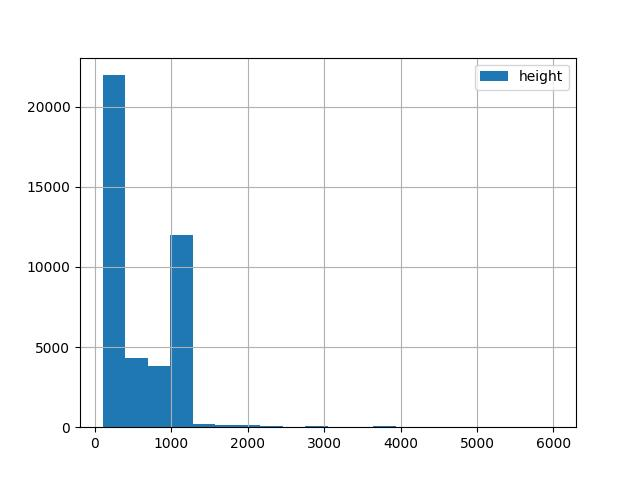
\includegraphics[width=0.9\textwidth, left]{"../visualizations/data_insights/Histogram of images height_original.jpg"}
	\end{subfigure}\hfill
	\begin{subfigure}{0.45\textwidth}
		\caption{"Histogram showing how frequent which width in the images are"}
		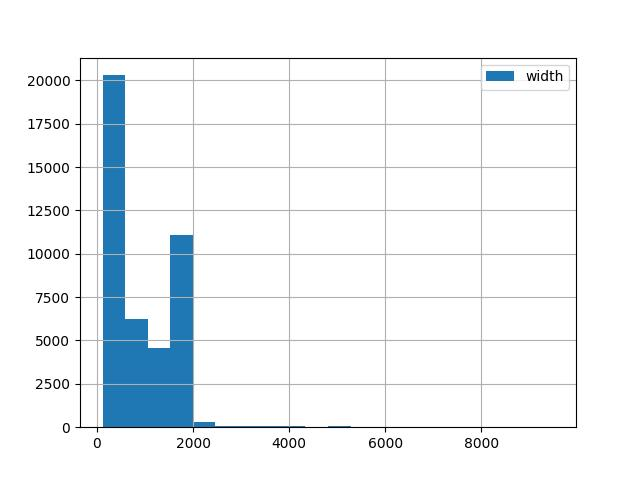
\includegraphics[width=0.9\textwidth, right]{"../visualizations/data_insights/Histogram of images width_original.jpg"}
	\end{subfigure}
\end{figure}
Most of the images appear to be quite small and having a look at the images together with these statistics they seem to be mostly quadratic. I wanted to take (256,256) as image size for training, but unfortunately I ran out of memory during training and had to decrease the image size to (128,128). Viewing some sample images from the datset shows that the size is still decent enough to have enough details. Although the picture in the first image showing candles does not really fit to the use case.\\
\begin{figure}[H]
	\centering
	\begin{subfigure}{0.9\textwidth}
		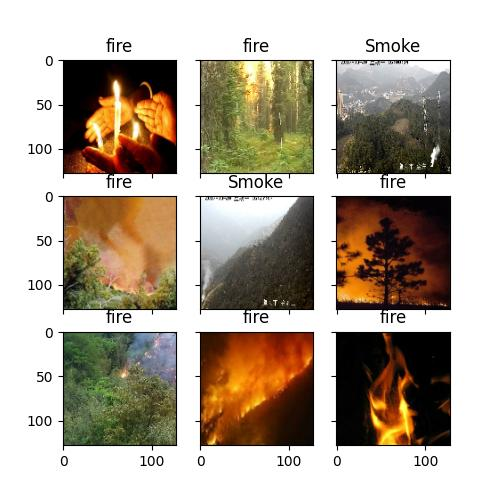
\includegraphics[width=0.9\textwidth]{"../visualizations/data_insights/sample_images1.jpg"}
	\end{subfigure}
	\begin{subfigure}{0.9\textwidth}
		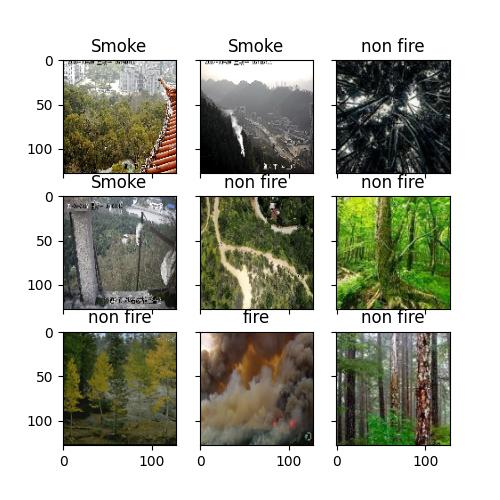
\includegraphics[width=0.9\textwidth]{"../visualizations/data_insights/sample_images.jpg"}
	\end{subfigure}
	\caption{"sample images from the dataset in the size (128,128)"}
\end{figure}
After starting the first training it became soon visible that not all images from the dataset could actually be used. A lot of them were *.tif files which TensorFlow could not handle and some were corrupted. So I took some code from a forum to filter the images out that are "bad". In the end mainly the "Smoke" class was influenced, but the dataset could still be called "balanced". So I did not take any measurements for handling imbalances. The width and height distribution did not change visually.\\
\begin{figure}[H]
	\centering
	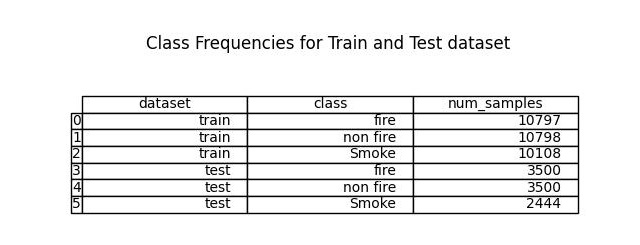
\includegraphics[width=0.9\textwidth]{"../visualizations/data_insights/class_frequencies.jpg"}
	\label{fig: class frequencies in test and train dataset}
\end{figure}

\section{Data Preprocessing}
All images were resized to (128,128).\\
Additionally in all models but the initial one I added a Rescaling Layer that rescales the image values from [0;255] to [0;1].\\
That was all preprocessing that happened.\\
\subsection{Data Augmentation}
For some of the models I started playing with Data Augmentation trying to get rid of the Overfitting of the models. For this I introduced a new function that creates a small data augmentation model which was applied to the training dataset. From all possible Ausmentations I just selected two. Random vertical Flipping and Random Rotation (but not too much). All other augmentations did not make sense in my eyes since they do not fit to the use case. Scaling the brightness per example would be unrealistic.\\

\section{Model Selection}
I trained in total 14 models trying different things to increase the accuracy of the models.\\
First I started with a rather big network having few layers only. Then in V2 I added the Rescaling and BatchNormalization layers which already increased the test accuracy. I wanted to test how the model behaves when I add some additional convolutional layers (V3). The accuracy did decrease on the test set. As compensation for the additional layers I tried to include Dropout layers with two different configurations (V4 + V5). This increased the networks test accuracy but was not much better than V2 with less convolutional layers. So I deleted the additional layer in V6, which gave me my best overall result with 0.976\% test accuracy. Still I had the feeling the model was overfitting as the training accuracy was extremly high. The test accuracy was of course as well high, but I had just this feeling as if the network was remembering the images as the validation accuracy was a little stagnating.\\
So I added data augmentation in V7 to see whether this would help a bit. And indeed the validation accuracy and train accuracy looked a little better as they were both increasing with the number of epochs. But unfortunately the overall training and testing accuracy went down. Model V8 can be omitted as there were no real new insights.\\
I removed the Data Augmentation again and got nearly competitive results with less filters in V9 although the test accuracy went down by 0.006\%. Still I wanted to see whether I could create a less complex model with the same accuracy. I decreased the number of filters in V10 and V11 and lost one percentage point of test accuracy. Hence I needed more filters again, but I did not want to increase the number of parameters again. So I added an additional convolutional layer in V12 which increased test accuracy again but could not match up with my "best" model until now. V13 and V14 were just tests to see how much i would need to decrease the number of parameters until I would be underfitting. Although I did not reach that goal I could see that the training accuracy did go down and I was unable to reach the good results from before.
\section{Best Results}
\section{Deployment}
\section{Further Steps}

\end{document}          
